\section{Implementation of Detection Algorithm}
\label{chap_implementation}
\subsection{Blocking WriteProcessMemory with a DACL}
\label{sec:implementation_dacl}
Most injection techniques call at some point in time the two important OpenProcess and WriteProcessMemory functions to inject into or modify in the remote process. It is not possible to easily intercept these calls from inside a user-mode process. One might try to prevent this function call and successful injecting from happening by just limiting the process access rights and removing the required permissions to call virtual memory modifying functions like WriteProcessMemory and ReadProcessMemory. The OpenProcess function will then not be able to return a handle with the required permissions. Implementing this approach works great in a test-application seen in [INSERT REF HERE], however once added to Google chrome, chrome malfunctions. Chrome relies heavily on inter process communication and therefore WriteProcessMemory and ReadProcessMemory are heavily used. Compiling chromium with the shown DACL Deny code results in a running executable that is at the end not fully functioning. The content of the browser is not displayed and opening web pages fails and immediately returns to the current open about:blank page. Therefore a different approach has to be taken to limit virtual memory modification.

\subsection{Blocking WriteProcessMemory with a kernelmode driver}
The newly created problem with the modified DACL can be solved by creating a driver running in kernel-mode. As reading memory, checking files and running processes are a common problem when writing anti virus software, Microsoft introduced object manager routines since Windows Vista to provide an efficient way of reacting onto these events. A driver would then use the ObRegisterCallbacks function to get notified whenever processes are created, files are opened and images (DLLs and EXEs) are loaded. This functionality offers the programmer to create a pre and post-execution callback function. Microsoft offers an example driver using ObRegisterCallbacks at \cite{github_obcallback} and shows how to modify the requested process handle permissions. In the provided example, the process will - as long as it is protected by the driver - not be terminated from outside. To protect chrome, the same actions described earlier will now be taken from inside the driver. Newly created process handles will be restricted to non virtual memory modifying permissions and the existing problem with inter process communication can be resolved by not restricting chromes child processes explicitly and give them a full access handle. [CODE REF] shows an implemented driver to fulfill the requirements. A demonstrational video of the resulting implementation can be found in the contained digital materials.

However, a naive implementation that just checks for process executables filename may result in access gain for the attacker. The  injecting process simply has to be named chrome.exe and can gain access to the original chrome.exe. However this implemented driver works and restricts outside access successfully. Children and parent processes ids (pids) are stored inside two separate tables that are on access checked if they contain target and source process ids. As memory managment is more difficult in kernelmode as dynamic memory allocation is a lot more advanced than in regular C/C++ applications, this driver uses a fixed size list structure. Finally the check for access rights can be done by finding a given pid inside the defined lists and returning a hash value which uniquely identifies the parent of the child process. Only if both find operations results match, access is then granted and no restriction is applied. Even though this implementation uses fixed size list, it is very efficient. During development an assumption regardings chrome process hierachy was made, so that only one parent process exists at the same time. If no further entries of chrome.exe parent processes exist, the find operation succeeds in at most 60 steps, but usually much faster. The find operation thus needs at least 11 iterations if the given process id is from a child process, because the list of all parents is crawled first.

\begin{figure}[ht]
\centering
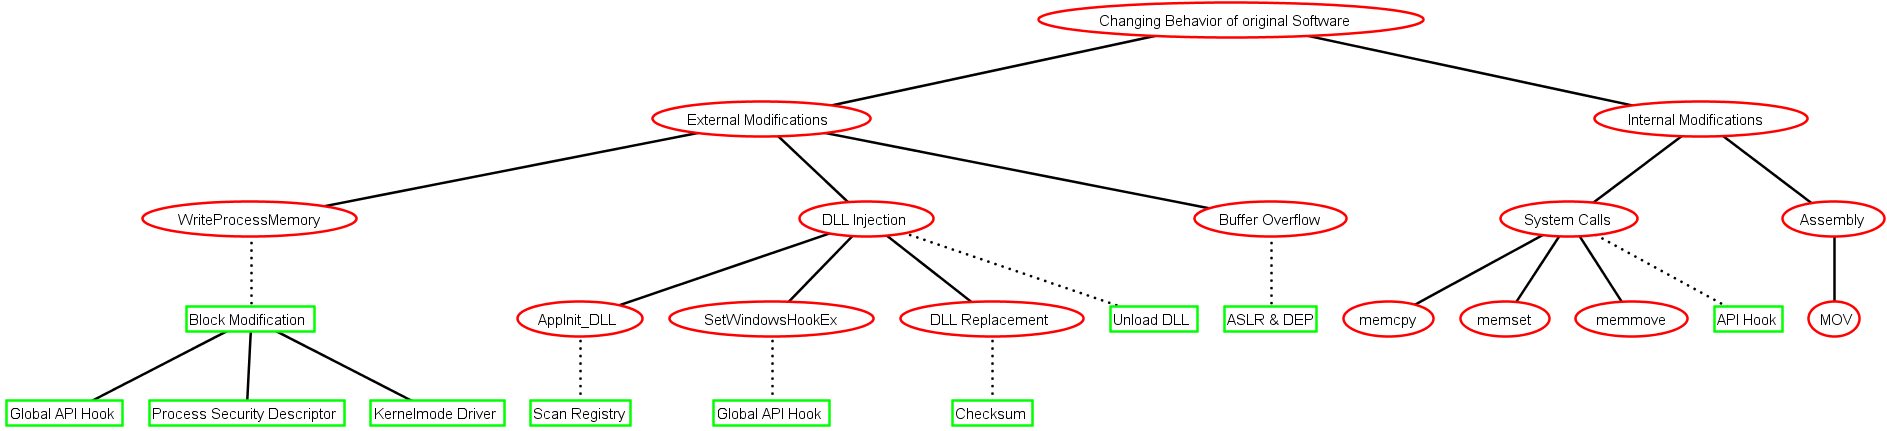
\includegraphics[width=\textwidth]{sections/adtrees/ProcessVirtualMemory.png}
\end{figure}